\documentclass{article}

\usepackage[utf8]{inputenc}
\usepackage[T1]{fontenc}
\usepackage{hyperref}
\usepackage{tabularx}
\usepackage{array}
\usepackage{fancyhdr}
\usepackage{graphicx}
\usepackage[a4paper]{geometry}
\usepackage{multicol}
\usepackage{listings}
\usepackage{pgfplots}

\pgfplotsset{width=10cm,compat=1.9}

\title{Apprentissage automatique \\ Le jeu de Nim}
\author{par Camille Leplumey et Geoffrey Spaur}
\date{03 Mai 2017}
\pagestyle{fancy}
\lhead{Apprentissage automatique - Le jeu de Nim \\ \textbf{M1GIL} - Camille Leplumey et Geoffrey Spaur}
\rhead{
\includegraphics[scale=0.5]{logo_univ_rouen.png}}
\setlength{\headsep}{1cm}
\begin{document}

\maketitle
\newpage
\tableofcontents{}
\newpage
\section{Mode \emph{easy}}
  \paragraph{}
    Le CPU joue aléatoirement sans prendre de décisions. Il est donc possible qu'il perde bêtement. 
    Le CPU jouera entre 1 et 3 bâtons comme indiqué dans les règles du jeu.
    Il lui sera cependant interdit de jouer 3 bâton alors qu'il en reste 2. Ainsi il jouera automatiquement 1 bâton, s'il reste 1 bâton en jeu.
    Et il jouera, avec 50\% de chance, 1 ou 2 bâtons quand il restera 2 bâtons en jeu.
\section{Mode \emph{medium}}
  \paragraph{}
    Le mode medium ne constitue en rien à de l'apprentissage. En effet nous codons les derniers coups que doit
    jouer le CPU. Le résultat sera donc identique à chaque parties sur les derniers coups et aléatoire sur les autres coups.
  \paragraph{}
    Dans notre cas le CPU jouera:
    \begin{itemize}
     \item 3 s'il reste 4 bâtons
     \item 2 s'il reste 3 bâtons
     \item 1 s'il reste 2 bâtons
    \end{itemize}
    Ormis c'est 3 cas spécifiques, le CPU jouera aléatoirement. Il est évident que le CPU jouera 1 s'il reste 1 bâton au même titre que dans le mode \emph{easy}.
    
\newpage
\section{Mode \emph{hard}}
  \paragraph{}
    Ici en entraînant le CPU contre lui même en mode \emph{hard}, il va apprendre la stratégie gagnante par lui même sans aide extérieur. 
    C'est un apprentissage \textbf{non supervisé}. Nous utilisons cette méthode car nous pouvons l'automatiser facilement.
  
  \subsection{Protocole des réalisations des graphiques}
  \paragraph{}
    Nous avons réalisé quelques statistiques concernant les différentes façons de jouer.
    Chaque points des courbes est une moyenne de 100 parties jouées. Chaque partie comprend une phase d'apprentissage,
    où le réseau de neurones se construira. Nous avons donc échelonné cette phase d'apprentissage pour réaliser nos graphiques.
    En conclusion le CPU apprendra sur 500 parties, nous effectuerons cet apprentissage 100 fois afin d'établir une moyenne de réussite.
    Nous procéderons de manière identique avec une phase d'apprentissage à 1.000 parties et ainsi de suite jusqu'à arriver à une phase d'apprentissage à 100.000 parties.
  \paragraph{}
    Il est important de remarquer nous notre échelonnage est \textbf{non proportionnel}. Il est donc possible de voir
    des légers paliers sur les différentes courbes des graphiques.
  
  \subsection{Graphique de réussite}
  \paragraph{}
    \begin{tikzpicture}
     \begin{axis}[
	title={Évolution du taux moyen de réussite entre 2 joueurs \textbf{hard} sans changement de rôle},
	ylabel={Taux de réussite en pourcentage },
	xlabel={Nombre de parties},
	ymin=0, ymax=100,ytick={0,20,40,60,80,100},
	xmin=0, xmax=7,xtick={0,1,2,3,4,5,6,7},
	xticklabels={0,100,500,1.000,5.000,10.000,50.000,100.000},
	scaled ticks=false,
	tick label style={/pgf/number format/fixed}, smooth,
	legend entries={Premier joueur,Second joueur},
	legend style={at={(0,1)},anchor=north west},
	legend cell align={left}
    ]
    
    \addplot[color=blue,mark=square,]
	coordinates {(0,50)(1,47)(2, 60)(3, 68)(4, 81)(5, 89)(6, 95)(7, 97)};
    \addplot[color=gray,mark=square,]
	coordinates {(0,50)(1,45)(2, 39)(3, 33)(4, 16)(5, 12)(6, 4)(7, 3)};
  
    \end{axis}
    \end{tikzpicture}\\
    Nous voyons ici qu'en jouant 800 parties, le CPU obtiendrais une moyenne de 65\% de réussite. De
    plus, nous pouvons affirmer qu'à partir de 50.000 parties jouées, le CPU ne fera quasiment plus d'erreurs.\\
    En théorie les deux courbes présentent sur ce graphique devrait être symétrique. Cependant nous avons effectué des moyennes 
    avec différent set de jeu. Cela explique l'asymétrie entre nos courbes.
    
  \subsection{Statistiques selon le mode de joueur}
  \paragraph{}
    \begin{tikzpicture}
     \begin{axis}[
	title={Évolution du taux moyen de réussite d'un joueur \textbf{easy} sans changement de rôle},
	ylabel={Taux de réussite en pourcentage },
	xlabel={Nombre de parties},
	ymin=0, ymax=100,ytick={0,20,40,60,80,100},
	xmin=0, xmax=7,xtick={0,1,2,3,4,5,6,7},
	xticklabels={0,100,500,1.000,5.000,10.000,50.000,100.000},
	scaled ticks=false,
	tick label style={/pgf/number format/fixed},
	legend entries={Second joueur easy,Second joueur medium,Second joueur hard},
	legend style={at={(0,1)},anchor=north west},
	legend cell align={left}
    ]
    \addplot[color=green,mark=square,]
	coordinates {(0,49)(1,49)(2, 51)(3, 50.5)(4, 50)(5, 50)(6, 50)(7, 50)};
    \addplot[color=blue,mark=square,]
	coordinates {(0,7)(1,5)(2, 6)(3, 6.5)(4, 6)(5, 6)(6, 6)(7, 6)};
    \addplot[color=red,mark=square,]
	coordinates {(0,50)(1,3)(2, 2)(3, 1)(4, 1)(5, 1)(6, 0.5)(7, 0.5)};
  
    \end{axis}
    \end{tikzpicture}
    
  \paragraph{}
    \begin{tikzpicture}
     \begin{axis}[
	title={Évolution du taux moyen de réussite d'un joueur \textbf{medium} sans changement de rôle},
	ylabel={Taux de réussite en pourcentage },
	xlabel={Nombre de parties},
	ymin=0, ymax=100,ytick={0,20,40,60,80,100},
	xmin=0, xmax=7,xtick={0,1,2,3,4,5,6,7},
	xticklabels={0,100,500,1.000,5.000,10.000,50.000,100.000},
	scaled ticks=false,
	tick label style={/pgf/number format/fixed}, smooth,
	legend entries={Second joueur easy,Second joueur medium,Second joueur hard},
	legend style={at={(0,0)},anchor=south west},
	legend cell align={left}
    ]
    \addplot[color=green,mark=square,]
	coordinates {(0,96)(1,95)(2, 94)(3, 94)(4, 95)(5, 95)(6, 95)(7, 95)};
    \addplot[color=blue,mark=square,]
	coordinates {(0,51)(1,51)(2, 49.5)(3, 50)(4, 50)(5, 50)(6, 50)(7, 50)};
    \addplot[color=red,mark=square,]
	coordinates {(0,95)(1,50)(2, 27)(3, 21)(4, 11)(5, 11)(6, 7)(7, 5)};
  
    \end{axis}
    \end{tikzpicture}
  \paragraph{}
    Sans surprise sur ces graphiques, nous ne voyons aucune évolution du taux de réussite contre les joueurs \emph{easy} et \emph{medium}, 
    car ces joueurs ne changent pas leur stratégie au cours du temps.
    Nous pouvons cependant constater de légère variation dans les premières parties due à un affinement de la moyenne.\\
    Il est à noté que le joueur \emph{hard} apprend plus vite en commeçant en second contre un joueur \emph{easy} que contre un joueur \emph{medium}.
    Cela souligne les différentes façons de jouer des joueurs \emph{easy} et \emph{medium}. Pour rappelle le joueur \emph{medium} joue aléatoirement tout comme 
    le joueur \emph{easy}, sauf pour le dernier coup, où le joueur \emph{medium} tentera de gagner.
  
  \paragraph{}
    \begin{tikzpicture}
     \begin{axis}[
	title={Évolution du taux moyen de réussite d'un joueur \textbf{hard} sans changement de rôle},
	ylabel={Taux de réussite en pourcentage },
	xlabel={Nombre de parties},
	ymin=0, ymax=100,ytick={0,20,40,60,80,100},
	xmin=0, xmax=7,xtick={0,1,2,3,4,5,6,7},
	xticklabels={0,100,500,1.000,5.000,10.000,50.000,100.000},
	scaled ticks=false,
	tick label style={/pgf/number format/fixed}, smooth,
	legend entries={Second joueur easy,Second joueur medium,Second joueur hard},
	legend style={at={(1,0)},anchor=south east},
	legend cell align={left}
    ]
    \addplot[color=green,mark=square,]
	coordinates {(0,50)(1,90)(2, 96)(3, 97)(4, 98)(5, 98)(6, 99)(7, 99.5)};
    \addplot[color=blue,mark=square,]
	coordinates {(0,5)(1,50)(2, 76)(3, 81)(4, 89)(5, 90)(6, 93)(7, 94)};
    \addplot[color=red,mark=square,]
	coordinates {(0,50)(1,47)(2, 60)(3, 68)(4, 81)(5, 89)(6, 95)(7, 97)};
  
    \end{axis}
    \end{tikzpicture}\\
    De loin le schéma le plus intéressant. En effet dans la phase 100 à 10.000 parties, nous pouvons voir que le joueur \emph{hard} commençant en premier, à un plus haut taux de réussite 
    contre un joueur \emph{medium}, que contre un second joueur \emph{hard}.
    Cela s'explique par le fait que le joueur \emph{medium} joue aléatoirement alors que le second joueur \emph{hard}
    essaye de découvrir la stratégie gagnante, tout comme le premier joueur \emph{hard}. Le premier joueur \emph{hard}, à partir des 10.000 parties
    perfectionne tellement son réseau que le second joueur \emph{hard} ne peut plus apprendre car il enchaînera les défaites.\\
    Il n'est donc pas surprenant de voir le taux de réussite contre un joueur \emph{medium} dépasser le taux de réussite contre un joueur \emph{hard} car 
    le joueur \emph{medium} ne peut pas se tromper sur le dernier coup contrairement au second joueur \emph{hard}.

  \subsection{Conclusion}
  \paragraph{}
    Pour conclure, si nous voulons jouer contre le CPU en mode \emph{hard}, il sera toujours possible de gagner.
    En effet le CPU choisi aléatoirement parmi ces connexions en favorisant les connexions à fort poids. 
    Néanmoins la chance que le CPU choisisse une connexion perdante sera toujours non nul, car les poids initiaux des connexions sont non nul et ne décroissent jamais. 
    Même si le CPU est bien entraîné, avec de la patience, il sera toujours possible de gagner une partie contre lui.


\newpage

\section{Proposition}
  \subsection{Agrégation}
  \paragraph{} 
    Nous avons remarqué que notre joueur \emph{hard} est quasiment imbattable s'il commence en premier,
    résultant du fait que nous l'avons entraîné à jouer en premier. Seulement nous pouvons remarquer que si ce joueur commence 
    en second sans entraînement préalable alors il sera aussi fort qu'un joueur en mode \emph{easy}.
  \paragraph{}
    Pour améliorer le joueur \emph{hard}. Nous avons donc pensé à créer 2 joueurs \emph{hard}. Le premier jouerai en premier contre en autre
    mode \emph{hard}. Le second jouerai en second contre un \emph{medium}. Les 2 joueurs résultant de cette apprentissage devrons être alors 
    agrégé afin que le joueur résultant soit capable de s'adapter à n'importe quelle situation, c'est-à-dire s'il commence en premier ou non.
  \paragraph{}
    Il sera cependant toujours possible de battre le réseau neuronal résultant, car le jeu de Nim admet une stratégie gagnante. Donc si vous connaissez cette stratégie
    et que vous commencer la partie toute en appliquant la stratégie gagnante, aucun réseau de neurones ne pourra vous battre.
  \paragraph{}
    Mais ici le but de notre réseau neuronal résultant est de reprendre la stratégie gagnante dans le cas où le joueur adverse commet une erreur.
    
  \subsection{Réduction des poids}
  \paragraph{}
    Une autre possibilité afin d’affiner notre réseau de neurone serait de \emph{punir} le chemin menant à la perte d'une partie.
    Cette \emph{punition} se traduirait par la réduction des poids des connexions empruntées par le chemin perdant.
    Il est cependant important de remarquer que si le poids d'une connexion tombe à 0, alors la connexion disparaît. Cela peut donc devenir problématique
    car le réseau neuronal pourrait s'enfermer dans des erreurs sans pouvoir se corriger.
  \paragraph{}
    Il est donc important que le poids d'une connexion ne tombe jamais à 0. Afin que le réseau puisse en permanence évaluer tout les cas
    possibles. C'est un processus obligatoire dans la correction d'erreurs. Cela implique - encore une fois - que le réseau ne pourra pas avoir un taux de
    réussite strictement égal à 100\%.
  
\end{document}